\documentclass[10pt,a4paper]{article}
\usepackage[utf8]{inputenc}

% \usepackage{ngerman}  % german documents
\usepackage{graphicx}  % import graphics einbinden
\usepackage{listings}  % support source code listing
\usepackage{amsmath}  % math stuff
\usepackage{amssymb} % 
\usepackage{a4wide} % wide pages
\usepackage{fancyhdr} % nice headers
\usepackage{float}
\usepackage{longtable}
\usepackage{xcolor}
\usepackage{booktabs}
\definecolor{darkpastelgreen}{rgb}{0.01, 0.75, 0.24}
\definecolor{spirodiscoball}{rgb}{0.06, 0.75, 0.99}
\definecolor{smalt}{rgb}{0.0, 0.2, 0.6}
\definecolor{armygreen}{rgb}{0.29, 0.33, 0.13}
\definecolor{awesome}{rgb}{1.0, 0.13, 0.32}
\definecolor{bittersweet}{rgb}{1.0, 0.44, 0.37}
\definecolor{bananayellow}{rgb}{1.0, 0.88, 0.21}
\definecolor{blue}{rgb}{0.0, 0.0, 1.0}
\definecolor{red}{rgb}{1.0, 0.0, 0.0}
\definecolor{green}{rgb}{0.0, 1.0, 0.0}

% for multiple figures
\usepackage{subcaption}


\lstset{basicstyle=\footnotesize,language=Python,breaklines=true,numbers=left, numberstyle=\tiny, stepnumber=5,firstnumber=0, numbersep=5pt} % set up listings
\pagestyle{fancy}             % header
\setlength{\parindent}{0pt}   % no indentation
 

\usepackage[pdfpagemode=None, colorlinks=true,  % url coloring
           linkcolor=blue, urlcolor=blue, citecolor=blue, plainpages=false, 
           pdfpagelabels,unicode]{hyperref}
           
% change enums style: first level (a), (b), (c)           
\renewcommand{\labelenumi}{(\alph{enumi})}
\renewcommand{\labelenumii}{(\arabic{enumii})}

\newcommand{\norm}[1]{\left\lVert#1\right\rVert}

%lecture name
\newcommand{\lecture}{
	Bioinformatics III
}           

%assignment iteration
\newcommand{\assignment}{
	Seventh Assignment
}


%set up names, matricle number, and email
\newcommand{\authors}{
  \begin{tabular}{rl}
    \href{mailto:s8tbscho@stud.uni-saarland.de}{Thibault Schowing} & (2571837)\\
    \href{mailto:wiebkeschmitt@outlook.de}{Wiebke Schmitt} & (2543675)
  \end{tabular}
}

% use to start a new exercise
\newcommand{\exercise}[1]
{
  \stepcounter{subsection}
  \subsection*{Exercise \thesubsection: #1}

}

\begin{document}
\title{\Large \lecture \\ \textbf{\normalsize \assignment}}
\author{\authors}

\setlength \headheight{25pt}
\fancyhead[R]{\begin{tabular}{r}\lecture \\ \assignment \end{tabular}}
\fancyhead[L]{\authors}


\setcounter{section}{7} % modify for later sheets, i.e. 2, 3, ...
%\section{Introduction to Python and some Network Properties} % optional, note that section invocation sets the section counter + 1, so adapt the setcounter command
\maketitle

%EXERCICE 1
\exercise{Missing Data Imputation}
All the listings are at the end of the exercise. 
\begin{enumerate}

% A
\item \textbf{The script}\\ 
\lstinputlisting[label=qtew-1, caption={Missing data imputation script}] {../Scripts/assignment7Part1.R}


%B
\item \textbf{Playing with the new mean and new standard deviation}\\

In figure \ref{fig:fig} we vary the mean and and standard deviation of the imputed data distribution. We can see the imputed data distribution sliding to the right when we change the new mean to a higher quartile and getting thinner when we take a smaller fraction of the original SD. The nicest fit is with one third of the original standard deviation and the 5\% quartile as the new mean (figure \ref{fig:sfig2}). In figure \ref{fig:rplacd} we show the distribution of the data after having replaced the NAs with the values generated with the same parameters as in figure \ref{fig:sfig2}.

\begin{figure}
	\begin{subfigure}{.5\textwidth}
		\centering
		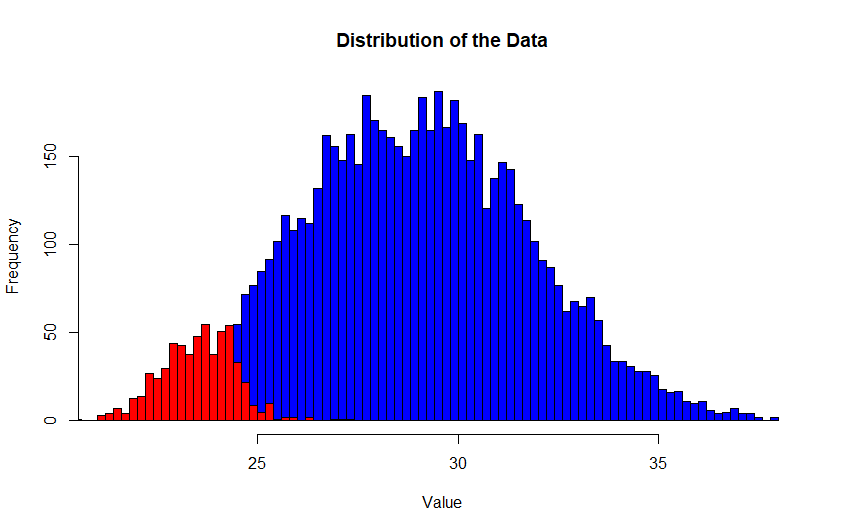
\includegraphics[width=.8\linewidth]{img/mean1sd13}
		\caption{New mean is the 1\% quartile of the data \\ distribution and SD is 1/3 of the original SD}
		\label{fig:sfig1}
	\end{subfigure}%
	\begin{subfigure}{.5\textwidth}
		\centering
		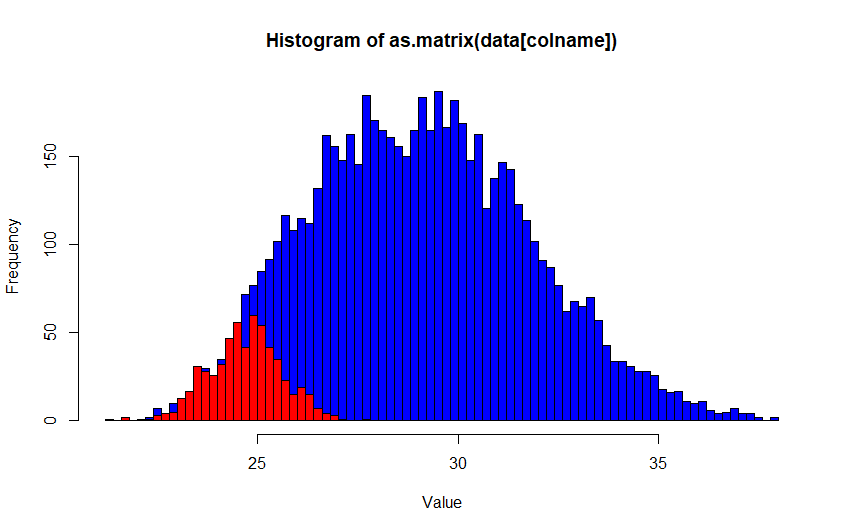
\includegraphics[width=.8\linewidth]{img/mean5sd13}
		\caption{New mean is the 5\% quartile of the data \\ distribution and SD is 1/3 of the original SD}
		\label{fig:sfig2}
	\end{subfigure}\\
	\begin{subfigure}{.5\textwidth}
		\centering
		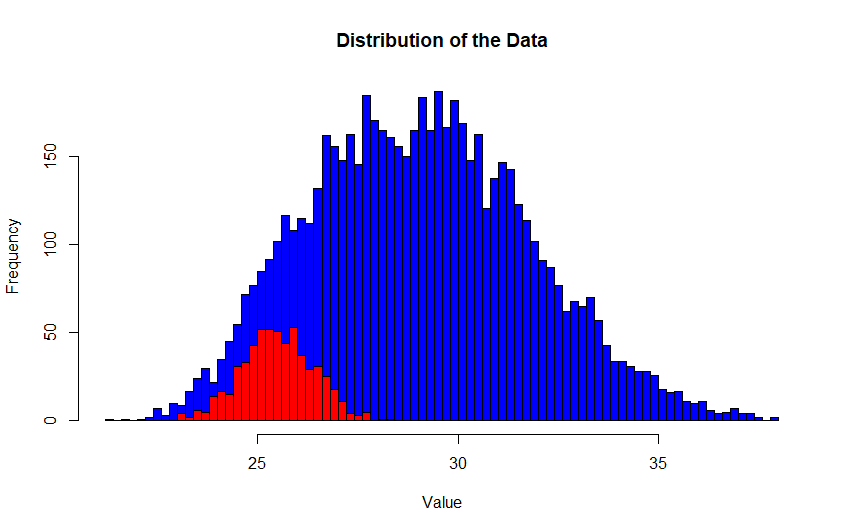
\includegraphics[width=.8\linewidth]{img/mean10sd13}
		\caption{New mean is the 10\% quartile of the data \\ distribution and SD is 1/3 of the original SD}
		\label{fig:sfig3}
	\end{subfigure}%
	\begin{subfigure}{.5\textwidth}
		\centering
		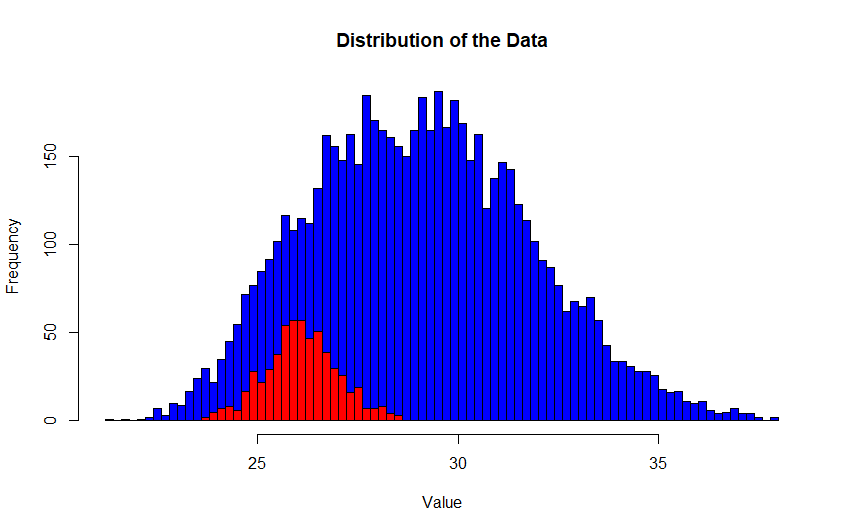
\includegraphics[width=.8\linewidth]{img/mean15sd13}
		\caption{New mean is the 15\% quartile of the data \\ distribution and SD is 1/3 of the original SD}
		\label{fig:sfig4}
	\end{subfigure}\\
	\begin{subfigure}{.5\textwidth}
		\centering
		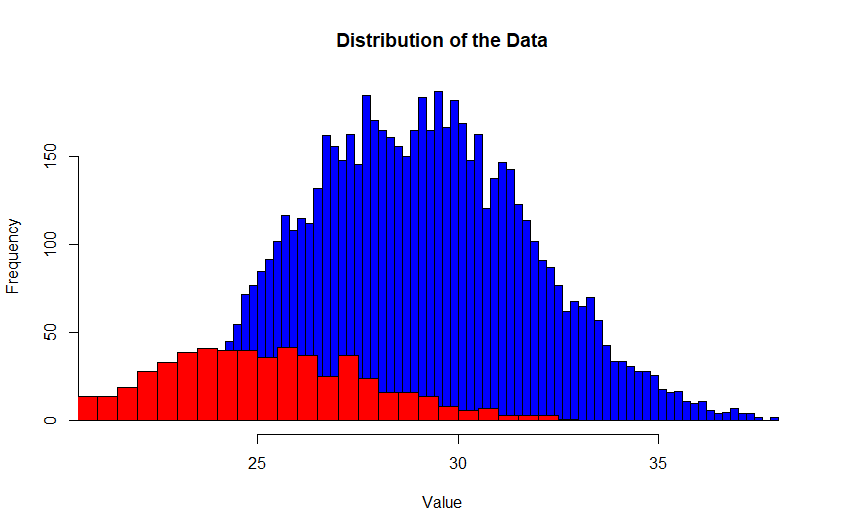
\includegraphics[width=.8\linewidth]{img/mean5sd1}
		\caption{New mean is the 5\% quartile of the data \\ distribution and SD is the original SD}
		\label{fig:sfig5}
	\end{subfigure}%
	\begin{subfigure}{.5\textwidth}
		\centering
		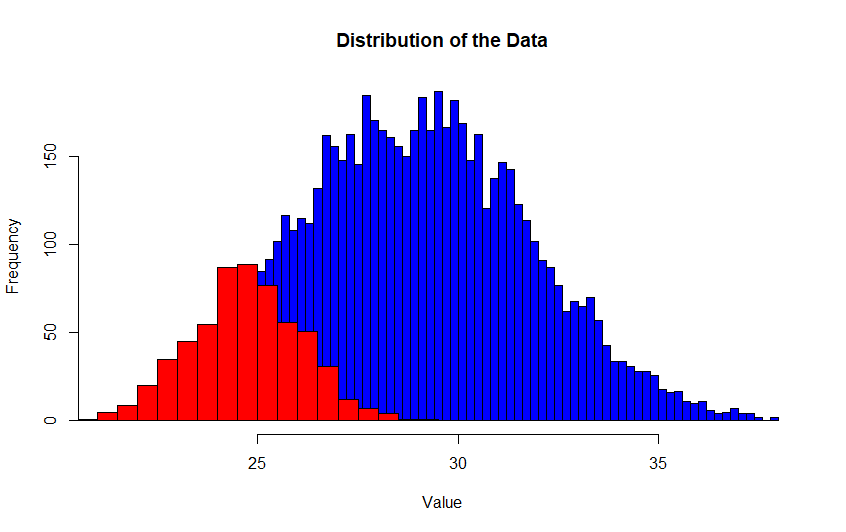
\includegraphics[width=.8\linewidth]{img/mean5sd12}
		\caption{New mean is the 5\% quartile of the data \\ distribution and SD is 1/2 of the original SD}
		\label{fig:sfig6}
	\end{subfigure}\\
	\begin{subfigure}{.5\textwidth}
		\centering
		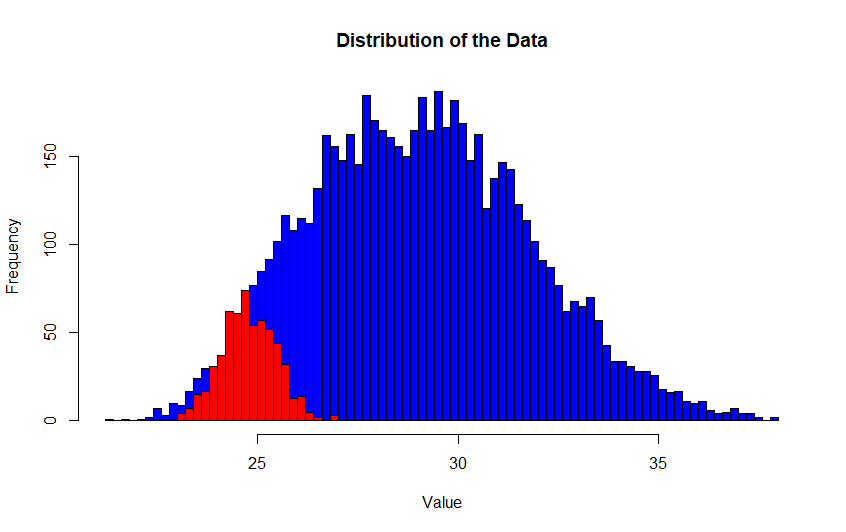
\includegraphics[width=.8\linewidth]{img/mean5sd14}
		\caption{New mean is the 5\% quartile of the data \\ distribution and SD is 1/4 of the original SD}
		\label{fig:sfig7}
	\end{subfigure}%
	\begin{subfigure}{.5\textwidth}
		\centering
		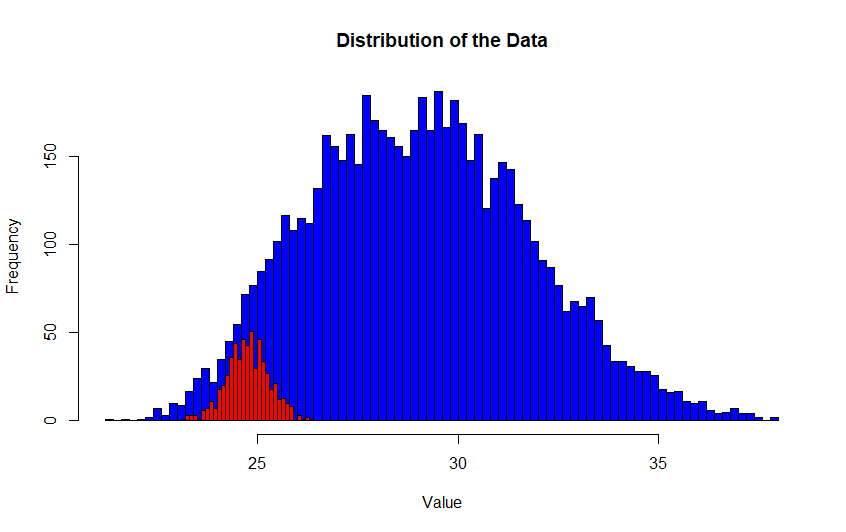
\includegraphics[width=.8\linewidth]{img/mean5sd15}
		\caption{New mean is the 5\% quartile of the data \\ distribution and SD is 1/5 of the original SD}
		\label{fig:sfig8}
	\end{subfigure}\\
	\caption{Variations of the new mean and the new standard deviation according to the one of the original distribution.}
	\label{fig:fig}
\end{figure}



\begin{figure}
	\centering
	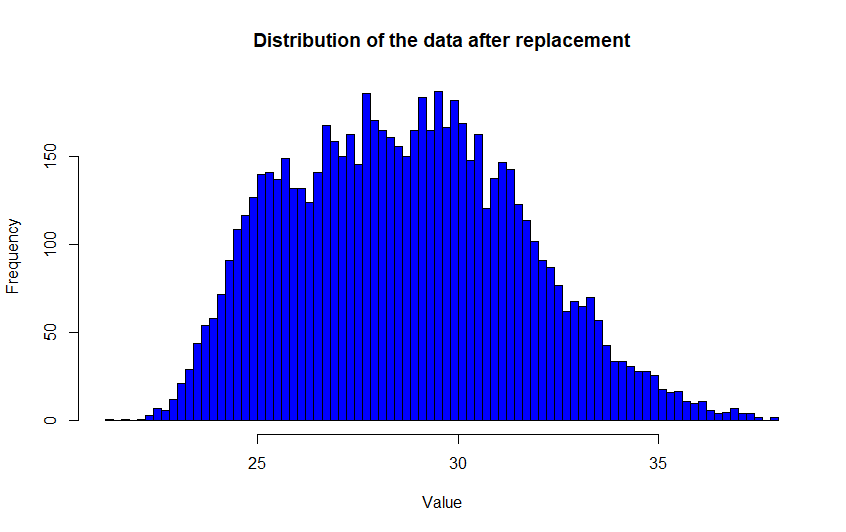
\includegraphics[width=0.7\linewidth]{img/rplacd}
	\caption{Data distribution after replacement of the NAs with the generated values.}
	\label{fig:rplacd}
\end{figure}



\end{enumerate}


%\newpage
%\lstinputlisting[label=qtew-1, caption={boolean\textunderscore network.py}] {../Scripts/boolean\string_network.py}
%\newpage
%\lstinputlisting[label=qtew-1, caption={Main function that tests the boolean network}] {../Scripts/main\string_boolean.py}




% NEW EXERCICE
\newpage
\exercise{DREAM challenge}
\begin{enumerate}
	
	% A
	\item \textbf{NOT IMPLEMENTED}\\

		%\lstinputlisting[label=lsdddt-1, caption={r}] {../ScriptsR/Assignment6Part2\string_schmitt\string_schowing.R}
	
	
	
\end{enumerate}

\end{document}